%Created by Fredrik Nilsson - freni169 with additions by Johan Billman - johbi142
\documentclass[12pt,a4paper]{article}
\usepackage[utf8]{inputenc}
\usepackage{alltt}
\usepackage[T1]{fontenc}
\usepackage[swedish]{babel}
\usepackage{mathtools}
\usepackage{lmodern}
\usepackage{units}
\usepackage{icomma}
\usepackage{color}
\usepackage{graphicx}
\usepackage{bbm}
\usepackage{tabularx}
\newcommand{\N}{\ensuremath{\mathbbm{N}}}
\newcommand{\Z}{\ensuremath{\mathbbm{Z}}}
\newcommand{\Q}{\ensuremath{\mathbbm{Q}}}
\newcommand{\R}{\ensuremath{\mathbbm{R}}}
\newcommand{\C}{\ensuremath{\mathbbm{C}}}
\newcommand{\rd}{\ensuremath{\mathrm{d}}}
\newcommand{\id}{\ensuremath{\,\rd}}
\usepackage{hyperref}
\usepackage[noindentafter]{titlesec}
\usepackage{color}
\usepackage{mathtools}
\usepackage{float}
\usepackage{longtable}

%Added stuff
\titleclass{\subsubsubsection}{straight}[\subsection]

\newcounter{subsubsubsection}[subsubsection]

\renewcommand\thesubsubsubsection{\thesubsubsection.\arabic{subsubsubsection}}
\renewcommand\theparagraph{\thesubsubsubsection.\arabic{paragraph}}
\renewcommand\thesubparagraph{\theparagraph.\arabic{subparagraph}}

\titleformat{\subsubsubsection}
{\normalfont\normalsize\bfseries}{\thesubsubsubsection}{1em}{}
\titlespacing*{\subsubsubsection}
{0pt}{3.25ex plus 1ex minus .2ex}{1.5ex plus .2ex}

\makeatletter
\renewcommand\paragraph{\@startsection{paragraph}{5}{\z@}%
	{3.25ex \@plus1ex \@minus.2ex}%
	{-1em}%
	{\normalfont\normalsize\bfseries}}
\renewcommand\subparagraph{\@startsection{subparagraph}{6}{\parindent}
	{3.25ex \@plus1ex \@minus .2ex}%
	{-1em}%
	{\normalfont\normalsize\bfseries}}
\def\toclevel@subsubsubsection{4}
\def\toclevel@paragraph{5}
\def\toclevel@paragraph{6}
\def\l@subsubsubsection{\@dottedtocline{4}{7em}{4em}}
\def\l@paragraph{\@dottedtocline{5}{10em}{5em}}
\def\l@subparagraph{\@dottedtocline{6}{14em}{6em}}
\makeatother

\makeatletter
\@addtoreset{subsubsubsection}{section}
\@addtoreset{subsubsubsection}{subsection}
\makeatother

\setcounter{secnumdepth}{6}
\setcounter{tocdepth}{6}
%End of new stuff


\DeclareGraphicsExtensions{.pdf,.png,.jpg}
\DeclarePairedDelimiter\abs{\lvert}{\rvert}%
\DeclarePairedDelimiter\norm{\lVert}{\rVert}%



% Swap the definition of \abs* and \norm*, so that \abs
% and \norm resizes the size of the brackets, and the 
% starred version does not.
\makeatletter
\let\oldabs\abs
\def\abs{\@ifstar{\oldabs}{\oldabs*}}
%
\let\oldnorm\norm
\def\norm{\@ifstar{\oldnorm}{\oldnorm*}}
\makeatother

\renewcommand{\abstractname}{Sammanfattning}


\setlength\parindent{0pt} %%NOINDENT



\title{TDDC74 -  Projektspecifikation}

\author{\textbf{Projektmedlemmar:}\\
Gustav Danielsson \small{gusda320@student.liu.se}\\
Marcus Dahlqvist \small{marda648@student.liu.se}\\ 
\bigskip\\ \textbf{Handledare:}\\
Jonas Wallgren {\small jonas.wallgren@liu.se}}

\date{\today}
\begin{document}
\maketitle
\newpage

\tableofcontents
\newpage

\section{Projektplanering}
Projektet går ut på att skapa ett actionspel där två eller fler spelare tävlar mot varandra. Spelet bygger på att med hjälp av tangentbordet styra ett flygplan på vald tvådimensionell spelbana. För att vinna skall man skjuta ner motståndarens flygplan och all information uppdateras grafiskt i realtid till de båda spelarna.

\subsection{Kort projektbeskrivning}
Programmet bygger på ett tvådimensionellt koordinatsystem med x och y axel. Objektens rörelse beskrivs med vektorer enligt linjäralgebraiska ekvationer där deras hastighet och riktning ska kunna vara påverkbara. Kollisionerna bygger på att få objekten att detektera om de är nära nog ett annat objekt då de aldrig kommer dela samma flytvärde. Skulle ett objekt vara för nära aktiveras eventet för kollision som att planet störtar eller plockar upp en form av buff. \\

Alla objekt ska även vara påverkade av ett gravitationsfält som läggs över koordinatsystemet som får att alla objekt kommer att falla mot marken om denna kraft inte motverkas i form av lyftkraft i någon form. Detta leder till att om man åker rakt upp för länge kommer spelaren tappa kontrollen över flygplanet och störta för en mindre tid baserat på gravitationskraften, tills det att hastigheten har stigit igen. \\

Programmet ska kunna hantera projektiler som ska kunna skjuta ner motståndare men även andra objekt som hindrar spelarens framfart. Dessa projektiler ska inte vara påverkade av gravitation. Detta är för att underlätta siktandet men även har en projektil i ett realistiskt scenario inte är märkbart påverkad av gravitation på så korta distanser. \\

Spelet ska även innehålla olika former av bonusar som kan plockas upp. Detta ger allt från en fartökning till nytt vapen eller liknande. Dessa ska kunna påverka planets beteende och dess rörelse i koordinatsystemet.  Även ska objekt kallat entities, som kan komma i form av till exempel fåglar eller luftballonger, kunna bli nedskjutna som kommer innehålla bonusar eller bara behöver bli förstörda så att man inte kolliderar med dem. 
Planet i sig ska kunna flyga i 16 olika riktningar för att ge en mjukare svängning samt ge fler riktningar att skjuta i så att spelaren har mer möjligheter att skjuta ner motståndaren. Vi svängning ska planet följa riktningen men även vridas runt x axeln för att ge en visuellt mer realistisk bild av att plant svänger. \\

Slutligen ska spelets inställningar kunna påverkas via en huvudmeny. Inställningarna består av val av spelbana, flygplan, antal poäng till vinst mm. Samt så ska spelet kunna pausas när en knapp trycks ned, och en pausmeny öppnas. Från denna meny ska man kunna återgå till spelet, avsluta pågående omgång eller avsluta programmet helt. \\


\subsection{Utvecklingsmetodik}
Vi strävar efter att genomföra det huvudsakliga arbetet i skolan på de erhållna tiderna. Vid behov försöker vi främst utnyttja lediga tider under arbetsveckan med vid behov även göra eget arbete hemma. Då båda medlemmarna har tillgång till laptop kan arbetet ske på valfri plats. Utöver det så ses vi dagligen samt har god kontakt vilket gör att kommunikation mellan medlemmarna kan ske utan stora förhinder. \\

Koden kommer att versionshanteras med tjänsten gitlab som kommer att underlätta konflikter med koden samt så erbjuder gitlab möjligheten att gå tillbaka till äldre versioner av koden vid olösliga problem.

\subsection{Grov tidplan}
I början kommer vi huvudsakligen att arbeta tillsammans för att få en bra struktur och en gemensam grundidé att arbeta utifrån. Vi strävar att få det gemensamma arbetet över så fort som möjligt då det går effektivare att arbeta individuellt. Sen utifrån grunden kan vi börja jobba mer individuellt på kommandon och olika grafiska delar som planens utseende till menyer eller finjustera fysikmotorn. Vi kommer dock ses regelbundet för att få en bättre bild av vad den andra personen gjort. På grund av att vi ses dagligen blir det även lätt att diskutera eventuella konflikter som uppstår vid individuellt arbete. \\

Vi kommer behöva bekanta oss med att arbeta med rackets inbyggda grafikpaket för att skapa menyer och spelet i sig. Samt så behöver vi lära oss att arbeta med realtidsuppdateringar och inte skapa ett spel som upplevs allt för ryckigt i manövreringen. \\

Till halvtidsmötet ska fysikmotorn och rörelsen i koordinatsystemet vara klart så spelet är fungerande fast utan grafik. Efter mötet kommer vi fokusera på att implementera grafiken och sedan relevanta funktioner när spelet har en grafik, såsom menyer, att kunna påverka vinstkriterier och avsluta spelet från en pausmeny.

\subsection{Betygsambitioner}
Då båda är intresserade av att göra ett så bra och givande projekt som möjligt siktar vi på att nå betyg 5. Vi båda arbetade på samma ingenjörsprojekt som byggde på att skriva ett reglertekniskt program och vi vill förbättra våra förmågor i utvecklandet av program ur ett projektperspektiv. 

\section{Användarmanual}
Programmet är sparat som Dogfight.exe och startas genom att köra filen. Vid start öppnas en start meny för att hjälpa spelarna förstå. \\

\begin{figure}[H]
	\caption{Bild som föreställer menyn i spelet}
	\centering
	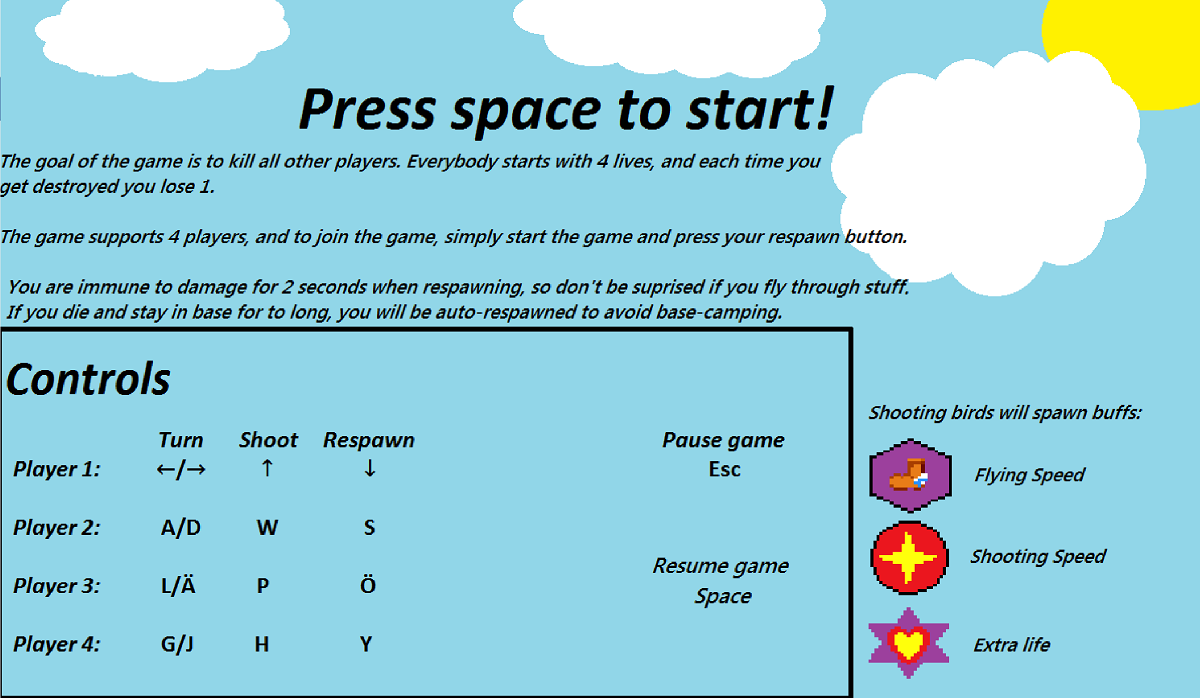
\includegraphics[width=\linewidth]{Dogfight_Menu_Example.png}
\end{figure}

Från Figur 1 kan all information som krävs för att kunna spela spelet erhållas. Alla spelares kontroller finns uppradade i controls rutan samt till höger om den en kort förklaring om hur de olika buffarna ser ut. Dessa erhålls som texten säger genom att skjuta ner fåglar. Reglerna för antal liv samt viktiga regler om hur respawning funkar erhålls ur texten över controls fältet. Vid tryck på space genereras spelbakgrunden och spelarna kan då börja tävla mot varandra. \\

\begin{figure}[H]
	\caption{Hur en spelomgång kan se ut}
	\centering
	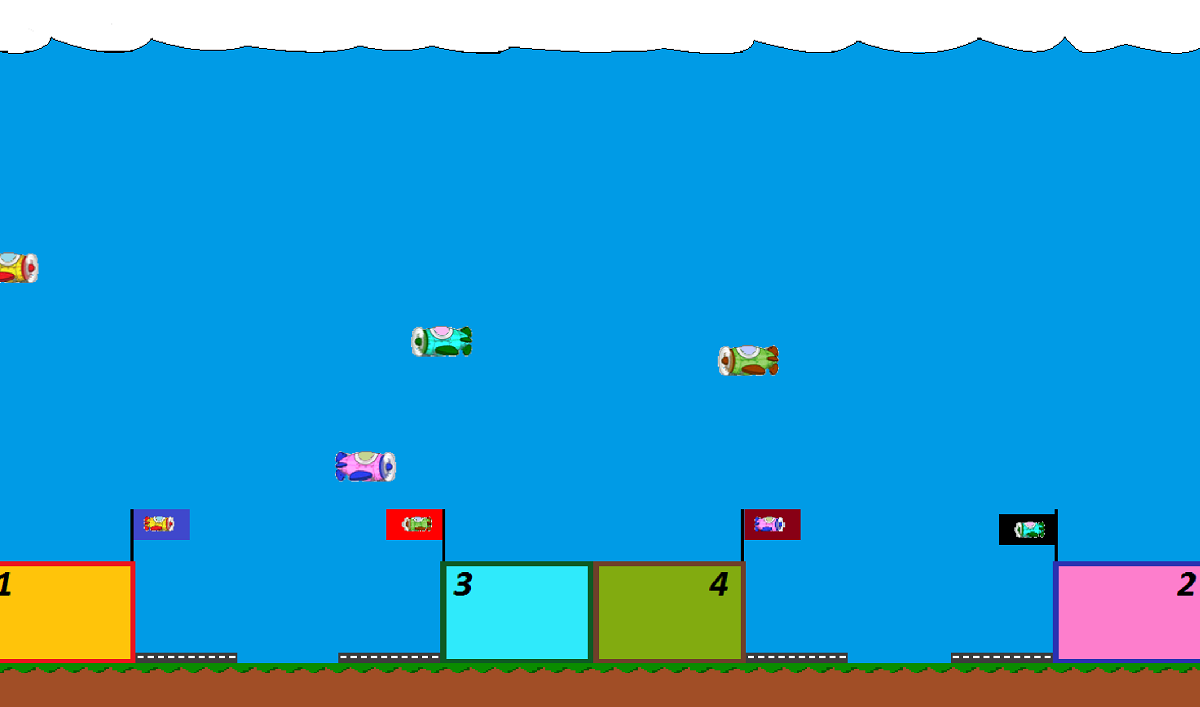
\includegraphics[width=\linewidth]{Dogfight_Ingame_Run_Exmple.png}
\end{figure}

Under en spelomgång kommer varje spelare som nämnts tidigare tilldelas 4 liv, dock kan fler erhållas genom att skjuta ner fåglar. Fåglar kommer att spawna från spelets kanter och åka tills de träffars av en projektil eller krockar i en vägg. Spelare kan åka in i kortsidan av spelplanen och komma tillbaka på andra sidan. Detta gäller dock ej för projektiler eller fåglar. Vid kollision kommer spelare att förlora liv samt kommer spelarens flagga sjunka korrensponderande med antalet liv kvar. Alla spelare kommer att respawna från sin hangar med dess nummer på. \\

Inga poäng erhålls från att skjuta ner någon utan det är en fråga om att inte krocka eller bli nerskjuten för att vinna. När alla andra spela har slut på liv vinner den sist levande spelaren. Vid det eventuella fallet att de två sista spelarna kolliderar är spelet oavgjort. När någon spelare har vunnit kommer man till en skärm som klargör vinnaren eller oavgjort och för att spela igen behöver programmet startas om igen. Viktigt att notera är att det krävs två splare för att ha en vinnare samt inget mer än att trycka på sin respawn knapp krävs för att vara med. Detta kan göras hela tiden tills en vinnare har valts. Spelet är därför rekkomenderat att spelas på minst två spelare för att få någon form av tävling med blir roligare med fler spelare då det blir mer hinder samt mer utmaning.

\section{Kravlista}
Här specificeras kraven för projektet. De lägre kravprioriteringarna 4-5 är inte nödvändiga, om implementeras snarare efter tillgänglig tid efter 1-3 är färdiga. 
\begin{longtable}{ | p{3.5cm} | c | c | p{3.5cm} | }
	\hline
	Krav & Prioritet & Kategori & Kommentar  \\ 
	\hline
	Världen ska byggas på ett tvådimensionellt koordinatsystem & 1 & Fysikmotor & \\
	\hline
	Det skall finnas objekt som kan ändra sin position i koordinatsystemet & 1 & Fysikmotor & \\
	\hline
	Positioner skall kunna uppdateras i realtid & 1 & Fysikmotor & \\
	\hline
	Objekt skall kunna förflyttas rakt i flera olika riktningar (16+) & 1 & Fysikmotor & Antal riktningar beror på vad som ger bäst spelupplevelse \\
	\hline	
	Objekt skall kunna ha olika storlek & 1 & Fysikmotor & \\ 
	\hline
	Objekt skall kunna kollidera med varandra & 1 & Fysikmotor & Exempelvis aktivering av en buff eller krascha mot marken \\ \hline
	
	Hastigheten för objekt skall vara varierbar & 2 & Fysikmotor & \\ 
	\hline
	Ett objekt som kolliderar med vänster/högerkant skall kunna komma fram på motsatt sida & 3 & Fysikmotor & \\ \hline
	Enkel gravitiation skall kunna simuleras & 3 & Fysikmotor & Kommer ungefär fungera så att objekt som rör sig uppåt kommer att få en lägre hastighet än de som rör sig nedåt. Kommer ej vara en konstant acceleration nedåt.\\ \hline
	Spelet skall kunna simulera vind  & 5 & Fysikmotor & \\ \hline
	Det skall vara möjligt att välja olika världar med annorlunda fysik & 5 & Fysikmotor & T.ex. välja att spela på månen med lägre gravitation eller liknande\\ \hline
	Det skall finnas spelarobjekt som kan styras av spelaren & 2 & Spelelement & \\ \hline
	Det skall  finnas en möjlighet för två spelare & 2 & Spelelement & \\ \hline
	Det skall finnas icke-spelarobjekt som spelaren kan interagera med & 2 & Spelelement & \\ \hline
	Det skall finnas ett markplan längst ned i världen & 2 & Spelelement & Vissa element kommer att elimineras vid kollision med marken\\ \hline
	Det skall finnas en himmel som gör att spelaren faller & 2 & Spelelement & Fungerar som ett tak fär spelplanen\\ \hline
	Spelaren skall kunna avfyra projektil-objekt  & 2 & Spelelement & Fungerar som vapen och kommer bland annat att kunna förstöra motspelare\\ \hline
	Det ska  finnas objekt som spelaren kan kollidera med som gör att spelaren kraschar & 2 & Spelelement & \\ \hline
	Det skall finnas ett vinst/förlustkriterie & 2 & Spelelement & I sin grund att skjuta ned motspelaren\\ \hline
	Vid för låg hastighet riktad uppåt skall spelarobjektet kunna förlora kontrollen & 2 & Spelelement & Planet faller rakt ned utan kontroll till en viss hastighet uppnås, varvid spelaren kan börja styra igen\\ \hline
	Om två spelare kolliderar med varandra skall båda krascha & 3 & Spelelement & \\ \hline
	Det skall finnas en plats där spelaren kan återuppstå & 3 & Spelelement & Kommer att vara i form av en landningsbana vid marken\\ \hline
	Vinst/förlustfunktionen ska utökas så att varje spelare har flera liv & 3 & Spelelement & \\ \hline
	Spelaren skall vara immun mot skada en kort tid efter återuppståndelse & 3 & Spelelement & För att undvika att motspelaren missbrukar den överlägsna positionen\\ \hline
	Spelaren skall ha tillgång till en aktiverbar hastighetsboost & 3 & Spelelement & Kommer att ha en tidsbegränsad aktiveringsfrekvens, som eventuellt kan förändras av bonusar\\ \hline
	Det skall finnas bonusar som spelaren kan aktivera & 3 & Spelelement & Kommer att göra saker som att öka maxhastighet, skjuthastighet m.m.\\ \hline
	Vid krasch ska spelaren störta mot marken, fortfarande med kollision & 4 & Spelelement & Det vill säga att andra objekt fortfarande kan kollidera med den till den når marken\\ \hline
	Det skall finnas stöd för upp till 4 spelare & 4 & Spelelement & \\ \hline
	Det skall vara möjligt att välja olika vinstkriterier & 5 & Spelelement & Detta skulle kunna vara: Tidsbegränsningar, fler liv, lagspel för 4 spelare.\\ \hline
	Man skall kunna starta spelet med 1 kommando & 1 & Användargränssnitt & Kommandot skall öppna en startmeny\\ \hline
	Det skall finnas en startmeny & 2 & Användargränssnitt & Skall innehålla instruktioner, start av spel och senare möjlighet att justera spelinställningar\\ \hline
	Det skall finnas en undermeny för instruktioner & 2 & Användargränssnitt & Här visas kontroller, vilka buffs som finns, och hur spelet går till\\ \hline
	Det skall finnas en knapp som startar huvudspelet i menyn & 2 & Användargränssnitt & \\ \hline
	Det skall finnas en knapp som avslutar spelet i huvudmenyn & 2 & Användargränssnitt & \\ \hline
	Huvudspelet skall kunna styras endast med ett tangentbord & 2 & Användargränssnitt & Kontrollerna som finns kommer att vara: Ändring av färdelseriktning medsols och motsols, avfyrning av vapen och aktivering av hastighetsboost\\ \hline
	Det skall finnas en knapp som avslutar spelet i huvudspelet & 2 & Användargränssnitt & \\ \hline
	Det skall finnas en knapp som pausar spelet & 3 & Användargränssnitt & i denna meny skall man kunna avsluta spelet eller återvända till huvudmenyn\\ \hline
	Menyn skall kunna navigeras endast med mus & 3 & Användargränssnitt & \\ \hline
	Det ska vara möjligt att själv ändra kontrollbindningarna i menyn & 5 & Användargränssnitt & \\ \hline
	Huvudspelet skall vara grafiskt implementerat & 2 & Grafik & \\ \hline
	Alla menyer skall vara grafiskt implemenerade & 3 & Grafik & \\ \hline
	Det skall finnas en indikator för antalet kvarstående liv & 3 & Grafik & \\ \hline
	Det skall finnas en indikator för hastighet & 4 & Grafik & \\ \hline
	Det skall finnas en indikator för kvarvarande tid till hastighetsbonus & 4 & Grafik & \\ \hline
	Det skall finnas en indikator för aktiverade bonusar & 5 & Grafik & \\ \hline
	Det skall finnas stöd för ljud i spelet & 4 & Övrigt & \\ \hline
	Ljud skall implementeras i huvudspelet & 4 & Övrigt & \\ \hline
	Det skall finnas musik i menyerna & 5 & Övrigt & \\ \hline
	Vid spelets slut skall statistik för matchen visas & 5 & Övrigt & Antal avfyrade skott, antal liv vid spelets slut, tidsåtgång, aktiverade bonusar, m.m.\\ \hline
\end{longtable}

\section{Implementation}
Här beskrivs ungefärligt processen under ett programvarv, samt de datatyper som kommer att användas av programmet. 

\subsection{Processbeskrivning}
Spelet kommer att uppdateras i realtid med någon lämplig uppdateringsfrekvens, där vilken framkommer med framtida tester. Vid en uppdatering kommer först alla objekt i rörelse att förflyttas beroende på deras riktning och hastighet. Steget efter detta är att detektera om några kollisioner har skett. Eftersom koordinatsystemet inte är i form av ett rutnät, så kommer positionerna istället komma att beskrivas av flyttal. Då sannolikheten att två objekt befinner sig på exakt samma flyttal vid samma tidpunkt är väldigt liten, så kommer objekten istället att ha en storlek, vilket innebär att kravet för kollision snarare blir att man jämför avståndet mellan två objekt och om den sammanlagda storleken är större än detta avstånd räknas det som en kollision.Om en kollision väl detekteras, kommer dess effekt att igångsättas efteråt, vilket till exempel skulle kunna vara aktivering av en buff eller en krasch. \\

Efter det att kollisioner har blivit behandlade, är nästa steg vara att avläsa spelarnas kommandon. Efter avläsning kommer sedan dessa värden sparas. De kommandon som finns är rotation medsols/motsols, avfyrning av projektil samt aktivering av hastighetsbuff. Värdena kontrolleras sedan för att se om de är tillåtna, vilket till exempel skulle kunna vara att spelaren nyss avfyrat en projekttil eller att spelaren störtar, och beroende på detta så kommer en åtgärd att utföras eller inte. \\

Nästa steg är att se om några nya objekt ska skapas, vilket antingen är en spelare som återuppstår eller ett icke-spelarobjekt som till exempel en fågel eller en buff. Objekt som spelare och bonusar kommer att skapas vid vissa händelser, medan fåglar och liknande kommer att skapas med någon form av slumpalgoritm. \\

Efter detta är ett programvarv färdigt för fysikmotorn, och det som är kvar är att uppdatera grafiken. Detta görs dock inte varje programvarv, utan kommer att göras med en frekvens på 60 Hz, och om tiden för detta inte är uppfylld så väntar programmet på att fysikmotorn ska uppdateras igen.

\subsection{Abstrakta datatyper}
I följande underrubrik beskrivs de olika datatyper och klasser som används i programmet.

\subsubsection{Flying-unit}
Datatypen \textbf{flying-unit} kommer att vara en överklass till alla flygande objekt, det vill säga spelare, hinder(exempelvis fåglar) och bonusar. Denna datatyp kommer även att representera projektiler som spelaren avfyrar, men då dessa projektiler inte har några extra egenskaper utöver de som beskrivs av \textbf{flying-unit}, så kommer denna klass att användas för att beskriva dem direkt.
\vspace{0.2cm}

\begin{tabular}{| c | c | p{8.3cm} |}
	\hline
	\textbf{Metod} & \textbf{Variabel} & \textbf{Beskrivning} \\
	\hline
	 
	 get-size & - & Returnerar bonusens storlek. \\
	 \hline
	 get-coordinates & - & Returnerar var spelaren befinner sig just nu. \\
	 \hline
	 get-direction & - & Returnerar åt vilken riktning spelaren är riktad åt i radianer.\\
	 \hline
	 get-speed & - & Returnerar vilken hastighet spelaren rör sig i.\\
	 \hline
	 set-coordinates! & \small\textbf{X Y} & Ändrar spelarens koordinater. \\
	 \hline
	 set-direction! & \small\textbf{angle} & Ändrar spelarens riktning. \\
	 \hline
	 set-speed! & \small\textbf{speed} & Ändrar spelarens hastighet. \\
	 \hline
\end{tabular}


\subsubsubsection{Player}
Datatypen \textbf{player} kommer att vara en klass som beskriver spelarobjekt, och kommer utöver de allmänna variablerna hos flygande objekt även att innehålla spelarobjektets unika egenskaper.

\vspace{0.2cm}

\begin{tabular}{| c | c | p{7.8cm} |}
	\hline
	\textbf{Metod} & \textbf{Variabel} & \textbf{Beskrivning} \\
	\hline
	
	get-size & - & Returnerar spelarens storlek \\
	\hline	
	get-max-speed & - & Returnerar spelarens tillåtna maxhastighet. \\
	\hline
	get-lives & - & Returnerar spelarens antal kvarstående liv \\
	\hline
	is-defeated? & - & Returnerar \#t om spelaren blivit besegrad, det vill säga inga liv kvar, och annars \#f. \\
	\hline
	can-fire? & - & Returnerar \#t om spelaren är tillåten att skjuta, annars \#f.\\
	\hline
	can-speedboost? & - & Returnerar \#t om spelaren är tillåten att använda speedboost, annars \#f. \\
	\hline
	is-plunging? & - & Returnerar \#t om spelaren har förlorat kontrollen på grund av för låg fart, eller kolliderat med toppen av spelplanen, annars \#f. \\
	\hline
	is-dead? & - & Returnerar \#t om spelaren är ur spel på grund av krasch, annars \#f. \\
	\hline
	set-max-speed! & \small\textbf{speed} & Ändras spelarens tillåtna maxhastighet. \\
	\hline
	set-lives! & \small\textbf{lives} & Sätter spelarens antal liv. \\
	\hline
	toggle-defeated! & - & Växlar om spelaren har blivit besegrad. \\
	\hline
	toggle-fire! & - & Växlar om planet är tillåtet att skjuta.\\
	\hline
	toggle-speedboost! & - & Växlar om planet är tillåtet att använda speedboost. \\
	\hline
	toggle-plunging! & - & Växlar om planet har förlorat kontrollen. \\
	\hline
	toggle-dead! & - & Växlar om spelaren är ur spel. \\
	\hline
	
\end{tabular}

\subsubsubsection{Buff}
Datatypen \textbf{buff} kommer att vara en klass som beskriver bonusobjekt, och kommer utöver de allmänna variablerna för flygande objekt även beskriva vilken typ av bonus det är. \\

\begin{tabular}{| c | c | p{8.2cm} |}
	\hline
	\textbf{Metod} & \textbf{Variabel} & \textbf{Beskrivning} \\
	\hline

	get-bonus-type & - & Returnerar vilken typ av bonus objektet är. \\
	\hline
	
\end{tabular}

\subsubsubsection{Entities}
datatypen \textbf{entities} kommer att vara en klass som beskriver flygande objekt som inte styrs av spelaren(exempelvis fåglar), och kommer förutom de allmäna egenskaperna för flygande objekt att beskriva de unika egenskaperna för dessa objekt. \\

\begin{tabular}{| c | c | p{9.5cm} |}
	\hline
	\textbf{Metod} & \textbf{Variabel} & \textbf{Beskrivning} \\
	\hline
	
	get-buff & - & Returnerar vilken typ av bonusobjekt som detta objekt lämnar efter sig vid kollision med en projektil, eller \#f om ingen lämnas.\\
	\hline
	
\end{tabular}

\subsubsection{World}
Datatypen \textbf{world} kommer att vara en klass som beskriver alla icke-rörliga kollisionsobjekt på spelplanen, det vill säga marken, himlen och landningsbanorna. \\

\begin{tabular}{| c | c | p{8cm} |}
	\hline
	\textbf{Metod} & \textbf{Variabel} & \textbf{Beskrivning} \\
	\hline
	
	get-coordinates & - & Returnerar vilka koordinater objektet har. \\
	\hline
	get-size & - & Returnerar objektets storlek. \\
	\hline
	get-type & - & Returnerar typen av kollisionsobjekt. Detta för att avgöra vilken åtgärd som ska utföras vid kollison, det vill säga förlust av kontroll för himmlen och krasch för mark och landningsbana. \\
	\hline
\end{tabular}

\subsubsection{Background}
Datatypen \textbf{background} kommer att beskriva den bakgrund vilket spelet spelas över, och även bakgrunden i menyerna. Denna kommer att vara statisk under spelets gång, och kommer därför bara att behöva uppdateras vid uppstart och när man går till menyn.

\vspace{0.2cm}

\begin{tabular}{| c | c | p{7cm} |}
	\hline
	\textbf{Metod} & \textbf{Variabel} & \textbf{Beskrivning} \\
	\hline
	
	choose-background & background & Ändrar vilken bakgrund som visas, exempelvis meny- eller huvudspelsbakgrund.\\
	\hline
	render & - & Börjar visa bakgrunden på skärmen. \\
	\hline
	hide & - & Slutar visa bakgrunden på skärmen. \\
	\hline
\end{tabular}

\subsubsection{Vector}
Datatypen \textbf{vector} kommer att beskriva vektorer och punkter i koordinatsystemet, om kommer bestå av ett par där car-delen är x-värdet och cdr-delen y-värdet.

\subsubsection{Matrix}
Datatypen \textbf{matrix} kommer att beskriva matriser som används för beräkningar, och kommer att bestå av en lista, där första elementet är en lista av första raden i matrisen, andra elementet är en lista av andra raden, etcetera.


\subsection{Testning}
När det gäller tester så är det främst viktigt att rörelserna i koordinatsystemet och kollisiondetekteringen fungerar på rätt sätt. Vi kommer därför att behöva testfunktioner som avläser och skriver ut de variabler som framkommer vid ett programvarv, för att se att saker får rätt position, att kollision detekteras korrekt samt att händelser kontrolleras och utförs korrekt. Lämpligt här är att skapa en testfunktion där programmet kan uppdateras med hjälp av ett knapptryck eller kommando istället för en klocka, för att på så sätt kunna analysera varje uppdatering på detaljnivå. Man bör även i kunna sätta alla variabler manuellt i testfunktionen, för att kunna testa specifika fall enklare. \\

Tidigt i implementeringen kommer vi främst att testa så att rörelser fungerar korrekt, så att föremål får rätt position i koordinatsystemet givet en riktning och en hastighet. När detta fungerar är huvudfokus att testa kollision av objekt och i sin tur att storlekar av objekt fungerar på rätt sätt. Här finns det även viktiga speciallfall att testa, till exempel om 3 objekt kolliderar med varandra under samma programvarv, då måste någon form av händelseprioritering göras. \\

Senare i projektet kommer även grafiken att behöva testas, men då fysikmotorn då redan ska vara implementerad handlar detta främst om att se så att kollisioner och liknande inträffar synkroniserat med att de grafiska objekten kolliderar. \\

\subsection{Beskrivning av implementation}



\section{Utvärderingar och erfarenheter}
    
Under projektet har ett antal motgångar dykt vilket gjort att det tagit mer tid att genomföra uppgiften än planerat vilket har lätt till att ett antal lågprioritetskrav har slopats. Dock har programmet från start haft en bra struktur och globala värden har undvikits vilket leder till att utökandet av spelare samt att göra nya funktioner har varit enkelt att implementera. Samt så har förbestämda sätt att bemärka funktioner, klasser, variabler och så vidare använts vilket gör programmet mer läsligt och sammanhanget blir bättre. Samt så har vi båda varit noga med att kommentera koden samt meddela när nya viktiga funktioner implementerats.  Att samarbetet funkat så bra har varit till stor hjälp vid problem med koden. \\

De huvudsakliga motgångarna i projektet har byggt på ambitionsnivå. Båda insåg när slutet närma sig att nivån som valts var för hög för att klara av på 160 timmars arbete var och var inte en rimlig nivå. Därför har några av de lågprioritetskraven slopats för att få ett bättre program med rimlig uppdateringshastighet samt mer rimlig arbetsbörda. Utöver det har en del av arbetsuppgifterna varierat i krav av insats vilket gjort att Marcus tagit på sig mer arbete till och från under projektets gång. \\

Dock så har projektet varit mycket givande för att ha en bättre inblick i hur man konstruerar större program där abstraktion på data behandlingen är ett krav. Båda projektmedlemmarna har jobbat på samma ingenjörsprojekt där koden var skriven på ett helt annat sätt vilket ledde till många bekymmer i optimeringsfasen av arbetet. Projektet har även gett ytterligare insyn i hur ett större program bör delas upp men även vad som är de mer krävande processerna. Detta gäller prestanda som antal timmar nerlagda för att skapa dem. Skulle ytterligare ett projekt göras av denna typ kommer vi ha bättre erfarenhet i hur arbetsbördan ska delas upp för att vara mer rättvis samt att inte köra fast då man väntar på att medarbetaren ska bli klar med sin kod. Detta leder annars till att mycket mer jobb måste göras de sista veckorna istället för att det flyter på med konstant hastighet hela projektet. \\


\end{document}